\begin{figure}[H]
\centering
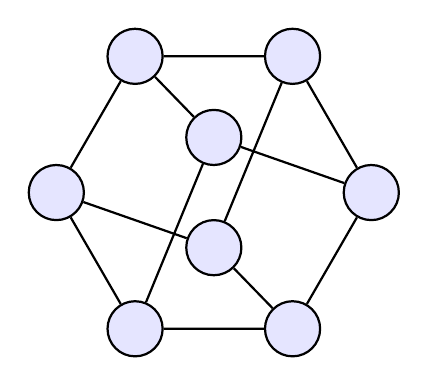
\begin{tikzpicture}[
  vnode/.style={circle, draw, minimum size=7mm, inner sep=0pt, fill=blue!10},
  thick
]
  % C6 cycle vertices (hexagon)
  \node[vnode] (v1) at (2, 0) {};
  \node[vnode] (v2) at (1, 1.73) {};
  \node[vnode] (v3) at (-1, 1.73) {};
  \node[vnode] (v4) at (-2, 0) {};
  \node[vnode] (v5) at (-1, -1.73) {};
  \node[vnode] (v6) at (1, -1.73) {};
  
  % Two internal vertices
  \node[vnode] (c1) at (0, 0.7) {};
  \node[vnode] (c2) at (0, -0.7) {};
  
  % Cycle edges (C6)
  \draw (v1) -- (v2) -- (v3) -- (v4) -- (v5) -- (v6) -- (v1);
  
  % Internal vertex c1 connects to v1, v3, v5
  \draw (c1) -- (v1);
  \draw (c1) -- (v3);
  \draw (c1) -- (v5);
  
  % Internal vertex c2 connects to v2, v4, v6
  \draw (c2) -- (v2);
  \draw (c2) -- (v4);
  \draw (c2) -- (v6);
\end{tikzpicture}
\caption{Příklad 3-regulárního grafu na 8 vrcholech ($C_6$ se dvěma vnitřními vrcholy).}
\end{figure}
